% Scalar instruction entry source: tools/generate_scalar_instruction_catalog.py.
\subsection{\texttt{SSRGET}}
\label{sec:scalar-ssrget}
\index{SSRGET@\texttt{SSRGET}}
\begin{sloppypar}\noindent\textbf{Purpose.} Reads a system register identified by the ID operand and writes the value to the selected destination.\end{sloppypar}\smallskip
\noindent\textbf{Syntax.}\par
\begin{lstlisting}[style=ptoscalarcode]
ssrget SSR_ID, ->RegDst
\end{lstlisting}
\noindent\textbf{Encoding.}\par
\noindent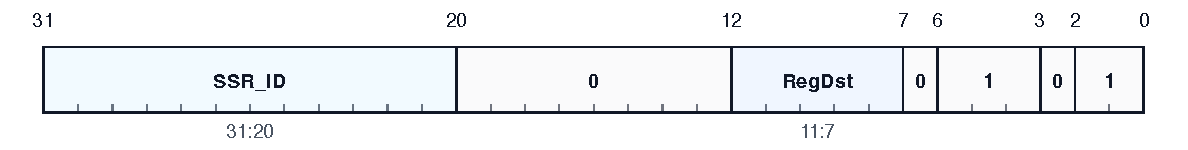
\includegraphics[width=\textwidth]{figs/encoding/scalar_instruction_entries/enc_ssrget.pdf}\par\smallskip
\begin{description}[leftmargin=0.18\linewidth,style=nextline]
\item[Format] \texttt{L32} \texttt{32-bit} scalar word.
\item[Pattern] \texttt{............00000000.....0111011}.
\end{description}
\noindent\textbf{Classification.}\par
\begin{description}[leftmargin=0.18\linewidth,style=nextline]
\item[Category] System, Cache, SSR, and Execution Control.
\item[Family] SSR Access.
\item[Execution class] \texttt{SYS}; uop\_kind=SYS, sys\_kind=SSR.
\end{description}
\noindent\textbf{Operand fields.}\par
\begin{description}[leftmargin=0.18\linewidth,style=nextline]
\item[\texttt{RegDst}] Bits \texttt{11:7 (5b)}. 5-bit scalar destination register written by this instruction; X0 is hardwired to zero, so writes to X0 are ignored.
\item[\texttt{SSR\_ID}] Bits \texttt{31:20 (12b)}. 12-bit system scalar register identifier selecting the SSR read, write, set, or swap target.
\end{description}
\noindent\textbf{Operation.}\par
\begin{lstlisting}[style=ptoscalarcode]
value = ReadSystemRegister(ID)
Write(RegDst, value)
\end{lstlisting}
\Needspace{0.08\textheight}
